\begin{framed}

Objetivos:
\begin{itemize}
    \item Entender por qué un perfil alar produce sustentación. 
\end{itemize}

Contenidos:
\begin{itemize}
    \item Repaso de superposición de flujos elementales para lograr un cilindro con sustentación.
    \item Flujos elementales con variable compleja. 
    \item La transformación de Joukowsky.
    \item La condición de Kutta.
    \item El vórtice de arranque.
\end{itemize}

Bibliografía:
\begin{itemize}
    \item White, F. M. (2008) Mecánica de Fluidos. McGraw-Hill. Sexta edición. Sección 8.4, 8.7.
    \item Batchelor, G. K. (2009) An Introduction to Fluid Mechanics. Cambridge University Press. Sección 6.7.
\end{itemize}
\end{framed}

\section*{Flujos elementales con variable compleja.}

En esta clase vamos a revisar una aplicación de flujo potencial: aerodinámica.
Hoy estudiaremos el flujo alrededor de perfiles alares, que son las responsables de que, por ejemplo, un avión se eleve.
Para esto, comenzaremos del análisis del flujo alrededor de un cilindro con sustentación, que estudiamos la clase pasada, y llegaremos a un perfil alar con una transformación topológica, lo que nos permitirá estudiar por qué un perfil alar produce sustentación con ecuaciones analíticas.

Antes de adentrarnos en aerodinámica como tal, nos conviene re-escribir las funciones de flujos elementales utilizando números complejos:
%
\begin{align}\label{eq:z_complejo}
z = x+iy\nonumber\\
\Phi = \phi + i\psi\nonumber\\
V = u+iv.
\end{align}

Usando las variables de la Ec. \eqref{eq:z_complejo}, podemos escribir los flujos elementales de manera equivalente a lo que ya conocemos:
%
\begin{itemize}
\item Flujo uniforme
%
\begin{align}\label{eq:flujo_uniforme_complejo}
\Phi_U &= U_\infty z\nonumber\\
       &= U_\infty (x+iy) = \phi_U + i\psi_U
\end{align}
%
\item Fuente
%
\begin{align}\label{eq:fuente_complejo}
\Phi_f &= \frac{q}{2\pi} \log(\overline{z})\nonumber\\
       &= \frac{q}{2\pi} \log\left(|z|e^{-i\theta}\right) = \frac{q}{2\pi} \left(\log(r) - i\theta\right) = \phi_f + i\psi_f
\end{align}
%
\item Vórtice
%
\begin{align}\label{eq:vortice_complejo}
\Phi_v &= -i\frac{\Gamma}{2\pi} \log(z)\nonumber\\
       &= -i\frac{\Gamma}{2\pi} \log\left(|z|e^{i\theta}\right) = \frac{\Gamma}{2\pi} \left(i\log(r) - \theta\right) = \phi_v + i\psi_v
\end{align}
%
\item Doblete
%
\begin{align}\label{eq:doblete_complejo}
\Phi_d &= \frac{K}{z} \nonumber\\
       &= \frac{K\overline{z}}{z\overline{z}} = \frac{K}{|z|^2}(x-iy)\nonumber\\ 
       &= \frac{K}{r^2}(r\cos(\theta) - i\sin(\theta)) = \phi_d + i\psi_d
\end{align}

\end{itemize}

Usar esta formulación nos simplificará mucho la vida a la hora de operar sobre dobletes y vórtices que no están centrados en el origen, ya que solamente hay que reemplazar $z$ por $z-z_0$, donde $z_0$ es el centro del vórtice, doblete o fuente.
Es más, podemos generalizar las expresiones de flujo uniforme y doblete a considerar una inclinación de éstos. 
Para un ángulo de inclinación $\alpha$, el flujo uniforme nos queda:
%
\begin{equation} \label{eq:flujo_uniforme_complejo_angulo}
\Phi_U = U_\infty z e^{-i\alpha}
\end{equation}
%
y el doblete
\begin{equation} \label{eq:doblete_complejo_angulo}
\Phi_d = \frac{K}{z}e^{i\alpha} 
\end{equation}

Utilizando números complejos, podemos calcular $\phi$ y $\psi$ de un flujo que entra en un ángulo $\alpha$ alrededor de un cilindro centrado en $z_0$ con una sola ecuación:
%
\begin{align} \label{eq:cilindro}
\Phi_\text{cil} = \phi_\text{cil}+i\psi_\text{cil} = U_\infty z e^{-i\alpha} + \frac{K}{z-z_0}e^{i\alpha} -i\frac{\Gamma}{2\pi} \log(z-z_0).
\end{align}

Por ejemplo, un flujo entrante con velocidad $U_\infty=1$ y $\alpha=8^\circ$ que pasa alrededor de un cilindro con radio $r=1.1$, centrado en $(-0.1,0)$ y con circulación $\Gamma=1$ tiene las siguientes líneas de flujo:
%
\begin{figure}\label{fig:flujo_cil}
\centering
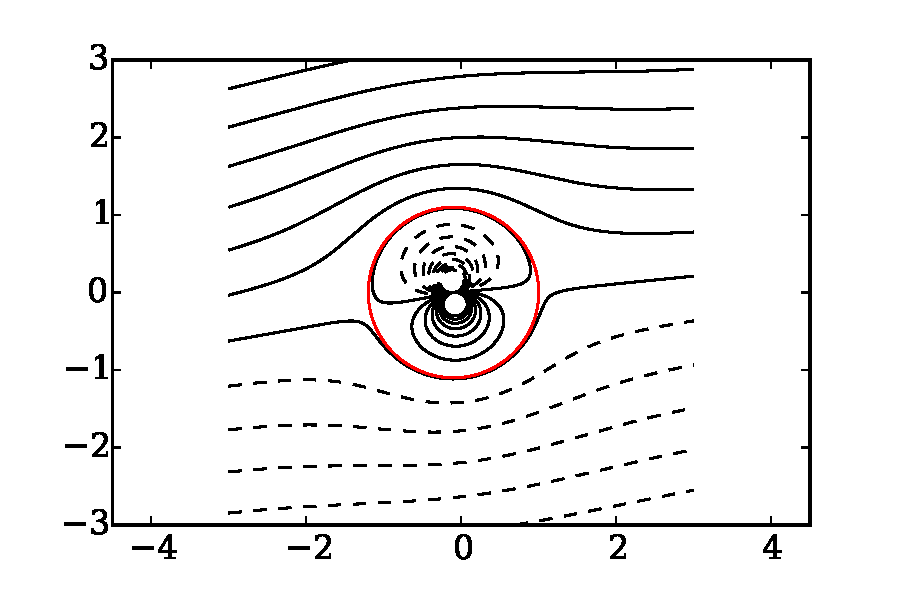
\includegraphics[width=0.7\textwidth]{clase05/flujo_cil.pdf}
\caption{Líneas de flujo alrededor de cilindro con circulación}
\end{figure}
%
y las líneas de equipotencial
%
\begin{figure}\label{fig:flujo_cil}
\centering
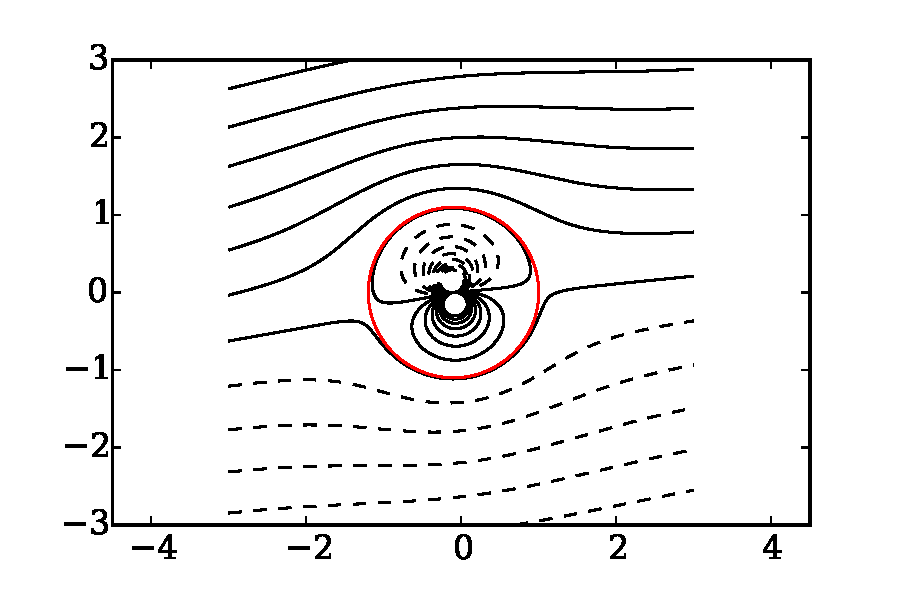
\includegraphics[width=0.7\textwidth]{clase05/flujo_cil.pdf}
\caption{Líneas de flujo alrededor de cilindro con circulación}
\end{figure}

Para calcular la fuerza del doblete ($K$) usamos el radio del cilindro, que de la clase anterior sabemos que es $r=\sqrt{K/U_\infty}$.

\section*{Transformación de Joukowsky}

La transformación de Joukowsky nos permite mapear un círculo a un perfil aerodinámico. 
Si $\zeta = \xi + i\eta$ son los puntos de un círculo en el plano $\zeta$, la tranformación de Joukowsky es
%
\begin{equation}
z = \frac{a}{2}\left(\zeta + \frac{1}{\zeta}\right)
\end{equation}
%
donde $z=x+iy$ son los puntos que definen el perfil aerodinámico, y $a$ es un factor que define el tamaño. 
Eso si, existe una condición: el contorno del círculo debe intersectar el punto $\xi=1, \eta=0$, y el punto $\xi=-1, \eta=0$ debe estar contenido dentro del círculo. 
De no cumplir estas condicones, la transformación genera geomterías que no se asemejan a un perfil aerodinámico.
